\documentclass{article}
\usepackage[english]{babel}
\usepackage[utf8]{inputenc}

% References and Bibliography
\usepackage[hidelinks]{hyperref}
\usepackage[natbibapa]{apacite}
\usepackage{natbib}
\bibliographystyle{apacite}

% align for equations
\usepackage{amsfonts}
\usepackage{mathtools}

% Table formatting
\usepackage{booktabs}

% Code blocks for Python
\usepackage{listings}
\usepackage{color}
\usepackage{inconsolata}

\definecolor{codegreen}{rgb}{0,0.6,0}
\definecolor{codegray}{rgb}{0.5,0.5,0.5}
\definecolor{codepurple}{rgb}{0.58,0,0.82}
\definecolor{backcolour}{rgb}{0.95,0.95,0.92}

\lstdefinestyle{CustomPython}{
	backgroundcolor=\color{backcolour},   
	commentstyle=\color{codegreen},
	keywordstyle=\color{magenta},
	numberstyle=\tiny\color{codegray},
	stringstyle=\color{codepurple},
	basicstyle=\footnotesize,
	breakatwhitespace=false,         
	breaklines=true,                 
	captionpos=b,                    
	keepspaces=true,                 
	numbers=left,                    
	numbersep=5pt,                  
	showspaces=false,                
	showstringspaces=false,
	showtabs=false,                  
	tabsize=2,
	basicstyle=\scriptsize\ttfamily
}

\lstset{style=CustomPython}

\newcommand{\documentlanguage}{english}  % Change to german if needed
\usepackage[autostyle=true]{csquotes}
\usepackage{multicol}
%\usepackage{natbib}
\usepackage{subcaption}
\usepackage[left=2.54cm,top=2.54cm,right=2.54cm,bottom=2.54cm,bindingoffset=0.5cm]{geometry}
\usepackage{gensymb}

\renewcommand\BBAA{and} % Kind of hacky
\renewcommand\BBAB{and} % But natbib citations forced me to do this :(
\DeclarePairedDelimiter{\norm}{\lVert}{\rVert}
\DeclarePairedDelimiter\abs{\lvert}{\rvert}
\begin{document}
\begin{otherlanguage}{\documentlanguage}
\begin{titlepage}
\begin{center}
	\vspace{3em}	
    {\Huge\bfseries DH2323 Computer Graphics and Interaction\par}
    \vspace{2em}
    {\huge Lab 2: Raytracing \par}
    \vspace{3em}
    {\Large Ramona Häuselmann\par}
    % {\Large ramonaha@kth.se\par}
	\vspace{1em}
    ramonaha@kth.se\\
	\vspace{1em}
    \today
\end{center}
\end{titlepage}
\newpage
\setcounter{page}{1}
\pagenumbering{arabic}
\section{Drawing Points} 
I used the given skeleton for the \texttt{Draw} function and implemented the \texttt{VertexShader} by using equations 3, 4 and 8 from the assignment instructions.
This resulted in the following image. We can see the vertex positions of the scene projected on the image as white pixels.
It looks the same as in the instructions.
\begin{figure}[ht]
    \centering
    
\includegraphics[width=10cm]{screenshots/drawing_points.png}
    \caption{Drawing Points}
\end{figure}

\section{Drawing edges}
I implemented the \texttt{Interpolate} function as given in the instructions and use it to draw a line as follows

\begin{lstlisting}[language=C++]
void DrawLineSDL(SDL_Surface* surface, glm::ivec2 a, glm::ivec2 b, glm::vec3 color) {
    glm::ivec2 delta = glm::abs(a - b);
    int pixels = glm::max(delta.x, delta.y) + 1;
    std::vector<glm::ivec2> line(pixels);
    Interpolate(a, b, line);
    for (int i = 0; i < line.size(); ++i) {
        PutPixelSDL(surface, line[i].x, line[i].y, color);
    }
}
\end{lstlisting}
Then I use the \texttt{DrawPolygonEdges} and \texttt{Draw} functions given in the instructions to 
create the image shown in Figure \ref{fig:DrawingEdges} a).
% \begin{figure}[ht]
%     \centering
%     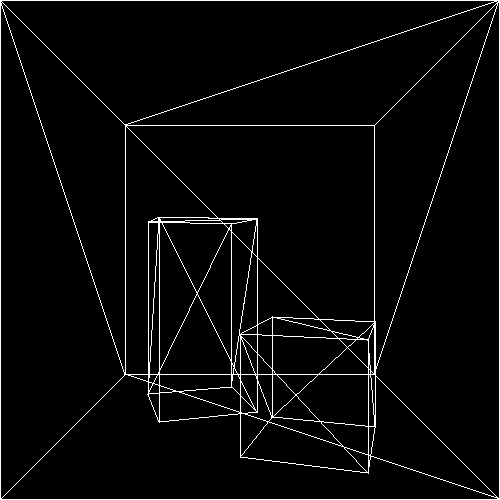
\includegraphics[width=10cm]{screenshots/drawing_edges.png}
%     \caption{Drawing Points}
% \end{figure}
I mapped W, A, S, D, Q, E to move the camera as follows:
\begin{itemize}
    \item W: move camera forwards
    \item S: move camera backwards
    \item D: rotate camera around y axis to the left (yaw)
    \item A: rotate camera around y axis to the right (yaw)
    \item Q: rotate camera around x axis down (pitch)
    \item E: rotate camera around x axis up (pitch)
\end{itemize}
I also implemented camera movement via mouse but I deactivated it for the rest of the assignment
since I found it a bit annoying.

\begin{figure}[ht]
    \centering
    \subfloat[Drawing Points]{
      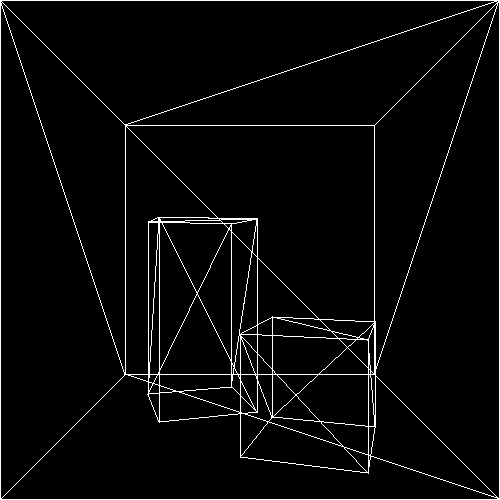
\includegraphics[width=\textwidth/2]{screenshots/drawing_edges.png}
    }
    \subfloat[Camera movement]{
      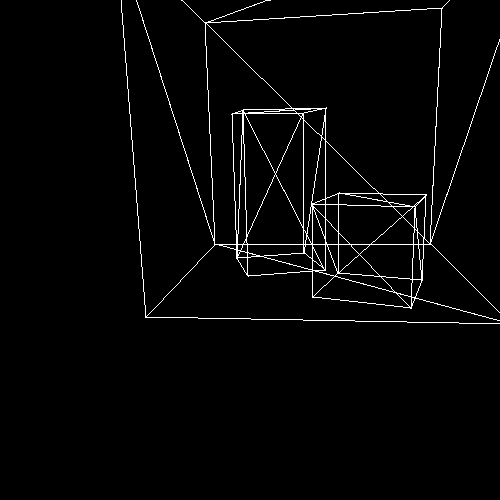
\includegraphics[width=\textwidth/2]{screenshots/drawing_edges_camera_movement.png}
    }
  
    \caption{Drawing Edges}
    \label{fig:DrawingEdges}
\end{figure}

\section{Filled Triangles}
I started with implementing \texttt{ComputePolygonRows} by implementing the given instructions in the comments.
To test my implementation I wrote \texttt{TestComputePolygonRows} to compare my output with the output
given in the instructions. While implementing this I had to debug some index out of bounds problems while
accessing my line vector but I was able to solve this after some debugging.
After I got that working I implemented the \texttt{DrawPolygonRows} function and finally used everything
to draw a the scene by using \texttt{DrawPolygon} and \texttt{Draw} as given in the instructions. This resulted in the image
shown in Figure \ref{fig:filledTriangles}, which looks the same as in the instructions. The blue box is overlapping the red box.

The rasterized scene in 500x500 pixel takes 5ms to render. The same scene raytraced takes 110ms.
We can see that rasterizing is much faster than ray tracing.
\begin{figure}[ht]
    \centering
    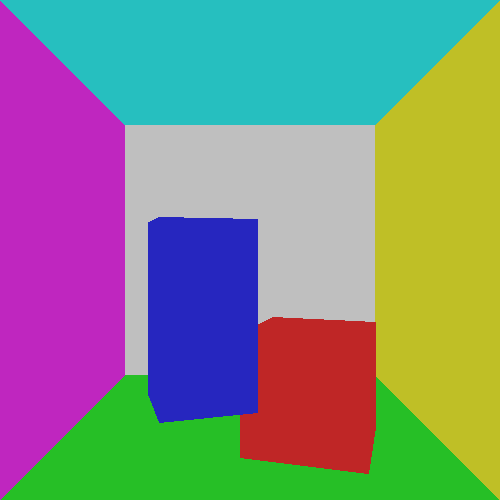
\includegraphics[width=10cm]{screenshots/filled_triangles.png}
    \caption{Filled Triangles}
    \label{fig:filledTriangles}
\end{figure}

\section{Depth Buffer}
I started by implementing an \texttt{Interpolate} function for \texttt{Pixel}s and calculate the \texttt{zinv}
value in the \texttt{VertexShader}. The \texttt{zinv} is interpolated over the triangle. In my \texttt{DrawLineSDL} function I then check the depth value
of the pixel before drawing. This results in the image shown in Figure \ref{fig:depthBuffer}.
Now the blue box does not overlap the red box anymore.
\begin{figure}[ht]
    \centering
    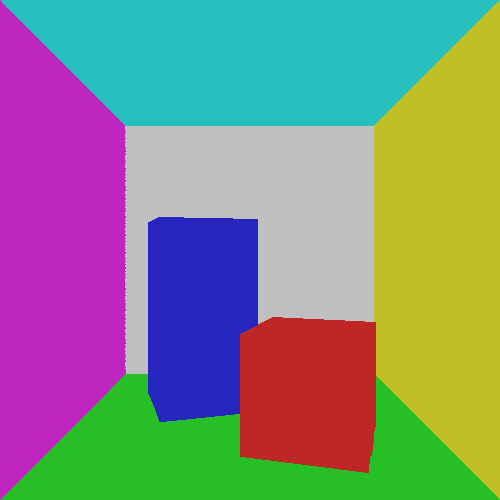
\includegraphics[width=10cm]{screenshots/depth_buffer.png}
    \caption{Depth Buffer}
    \label{fig:depthBuffer}
\end{figure}

\section{Illumination}
I started by implementing and adjusting \texttt{PixelShader} and \texttt{VertexShader} as given in the instructions.
After adding the calculations described in the instructions I get the result in Figure \ref{fig:perVertexIll}. 
Here we calculate the illumination per vertex and interpolate the illumination over the triangles.
\begin{figure}[ht]
    \centering
    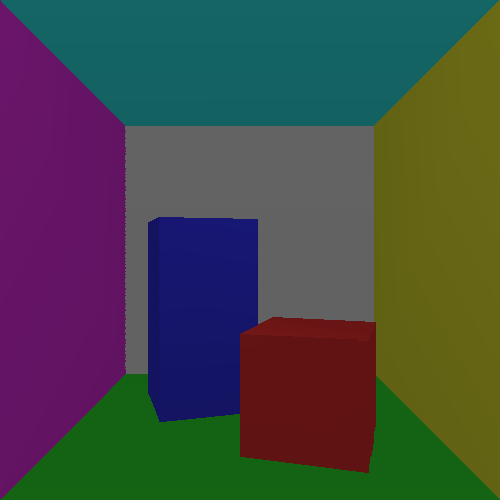
\includegraphics[width=10cm]{screenshots/per_vertex_illumination.png}
    \caption{Per vertex illumination}
    \label{fig:perVertexIll}
\end{figure}
Figure \ref{fig:perPixelIllSkewy} shows the result after adjusting the code to use per pixel illumination. Here we interpolate the 3D position
over the triangle and use this interpolated position to calculate the illumination of each pixel.
\begin{figure}[ht]
    \centering
    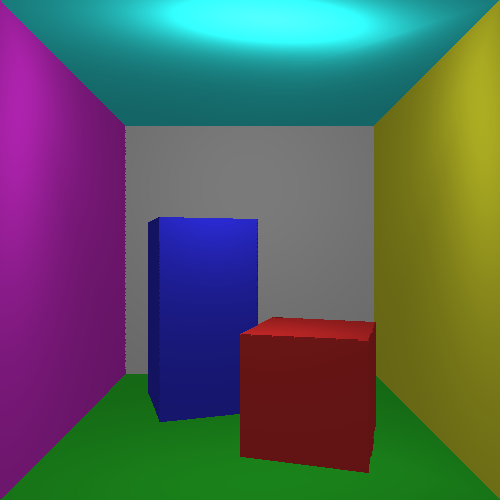
\includegraphics[width=10cm]{screenshots/skewy_per_pixel.png}
    \caption{Per pixel illumination (skewy)}
    \label{fig:perPixelIllSkewy}
\end{figure}
In Figure \ref{fig:perPixelIllSkewy} the illumination looks skewy since we are not using perspective correct
interpolation. By interpolating over p/z instead of 1/z we obtain the correct looking illumination 
shown in Figure \ref{fig:perPixelIllNotSkewy}.
\begin{figure}[ht]
    \centering
    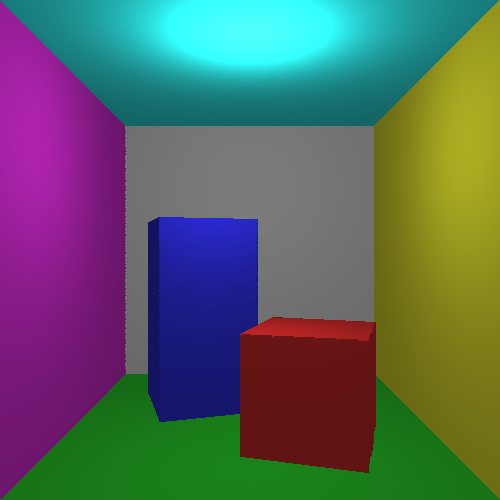
\includegraphics[width=10cm]{screenshots/per_pixel_notskewy.png}
    \caption{Per pixel illumination (not skewy)}
    \label{fig:perPixelIllNotSkewy}
\end{figure}
Finally I added light movement with the following mapping: 
\begin{itemize}
    \item UP: move light forwards
    \item DOWN: move light backwards
    \item LEFT: move light to the left
    \item RIGHT: move light to the right
    \item RIGHT\_SHIFT: move light up
    \item RIGHT\_CTRL: move light down
\end{itemize}
Figure \ref{fig:moveLight} shows the scene with a different light position.
\begin{figure}[ht]
    \centering
    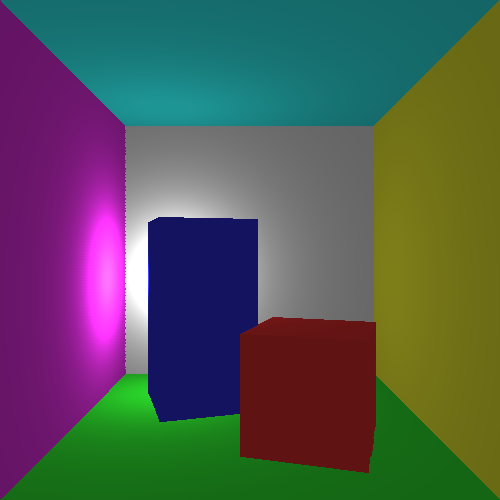
\includegraphics[width=10cm]{screenshots/move_light.png}
    \caption{Move light}
    \label{fig:moveLight}
\end{figure}
\end{otherlanguage}
\end{document}
